\documentclass[a4j,11pt]{jsarticle}
\usepackage{semi}
\usepackage{breqn}
\usepackage{tabularx}
\usepackage{listings,jlisting}

\lstset{
  basicstyle={\ttfamily},
  identifierstyle={\small},
  commentstyle={\smallitshape},
  keywordstyle={\small\bfseries},
  ndkeywordstyle={\small},
  stringstyle={\small\ttfamily},
  frame={tb},
  breaklines=true,
  columns=[l]{fullflexible},
  numbers=left,
  xrightmargin=0zw,
  xleftmargin=3zw,
  numberstyle={\scriptsize},
  stepnumber=1,
  numbersep=1zw,
  lineskip=-0.5ex
}

\newcolumntype{Y}{&gt;{\centering\arraybackslash}X} %中央揃え
 
\makeatletter % プリアンブルで定義開始

% 図番号を"<章節などの番号番号> - <図番号>" へ
\renewcommand{\thefigure}{\thesubsection-\arabic{figure}}
\renewcommand{\thetable}{\thesubsection-\arabic{table}}
% 章が進むごとに図番号をリセットする
\@addtoreset{figure}{subsection}
\@addtoreset{table}{section}
\renewcommand{\theequation}{% 式番号の付け方
	\thesection.\arabic{equation}}
	\@addtoreset{equation}{section}
\makeatother % プリアンブルで定義終了

\renewcommand{\headfont}{\bfseries} %章タイトルなどを明朝体にする

\makeindex
\begin{document}
\definecolor{cellcolor}{rgb}{ 1, .90, .90}
\definecolor{rowcolor}{rgb}{.85, .85, 1}
\setcounter{tocdepth}{3}
\thispagestyle{empty}
\clearpage
\addtocounter{page}{-1}
\begin{center}

\huge
2019年度 卒業論文\\[70pt]
\HUGE
主体性を養う反転授業の提案\\[70pt]
\huge
指導教員 須田 宇宙 准教授\\[50pt]
千葉工業大学 情報ネットワーク学科\\[20pt]
須田研究室\\[40pt]
1632024 \hspace{70pt} 植本 匠海\\[110pt]
\end{center}
\begin{flushright} 
\huge

\textcolor{white}{文字}

\textcolor{white}{文字}

提出日 2020年1月30日
\end{flushright}
\newpage
\pagestyle{empty}
\clearpage
\addtocounter{page}{-1}
\large
% 目次
\tableofcontents
\thispagestyle{empty}
\clearpage
\pagestyle{plain}
\newpage

%表目次
\listoftables
%図目次
\listoffigures
\thispagestyle{empty}
\addtocounter{page}{-1}
\newpage

\addtocounter{page}{-1}
\section{緒言}

近年では,時代の変化がとても早い中で主体性を持ち自ら学び,考え,行動できる人材が必要とされている.しかし,教育の場で受動的な学習が行われている.その原因の1つとして学生の主体性が低いことが挙げられる.また,主体性を向上させる新しい学習方法のブレンド型学習の一つとして,自宅などで基礎知識を学んだあとに,課題や応用を授業時間内に行う反転授業が注目されている.

しかし,三田の研究では授業前までに見てもらう予習動画をすべて見た学生が3割以下であることや\cite{1},大谷らのグループ学習を取り入れた研究では主体性が高い学習者のみで進めてしまい,その他の学習者が積極的に参加しなくても授業が進んでしまっていることなど\cite{2},学習者それぞれの主体性の違いが問題点として報告されている.

そこで本研究では,反転授業のグループ学習において,一人一人の学生に責任ある立場に付かせてグループワークを行ってもらい,主体性に変化があったかを分析することを目的とする.
\newpage

\section{主体性}
主体性とは自分の意志で行動しようとする態度である\cite{3}.

\subsection{現代における主体性の必要性}
経済産業省は,平成29年度に開催した「我が国産業における人材力強化に向けた研究会」において,さらに長くなる個人の企業・組織・社会との関わりの中で活躍し続けるために求められる力を「人生100年時代の社会人基礎力」と定義した\cite{4}.この中の「前に踏み出す力」の1つとして,主体性があり「指示待ちにならず,一人称で物事を捉え,自ら行動できるようになることが求められている.」とされている.

また,日本経済団体連合会の「高等教育に関するアンケート結果」\cite{5}で,「学生に求める資質,能力,知識」について企業が「主体性」「実行力」「協調性」など複数項目の中から上位5つを選択してもらったところ,文系・理系学生ともに主体性が1位であった.

このように現在働いている人達だけでなく,これから社会に出る学生にも主体性は求められている.

\subsection{学生の主体性}
大学生の学習などについての調査報告書\cite{6}によると,現在の大学生が主体性を持って学習をしているとは言い難い.8年間の意識の変化では,授業の内容よりも授業の単位の取得のし易さで授業を選ぶ学生が約12\%増加し61.4\%に増えている.また,自分で工夫して学習するよりも授業で指導を受けたほうがよいという学生は約11\%増加し50.7\%に増えている.このように,受動的な学習をしてしまう学生が増加している.

社会では主体性のある学生の必要度が増加しているのに対して,現状は残念ながら主体性がある学生が減少してきている.



\newpage

\section{授業形態}
\subsection{従来型授業}
現在日本の多くの教育の場で行われているのが,授業時間内に基礎的な知識を学んだあとに,授業時間外に応用の問題に取り組むというものである.教員が教科書を用いて学習者に対して,その単元の基本的な知識を解説する.これは座学に分類され教員が学習者に対して,一方的な物となっている.授業で基礎を学んだあとに,自宅などで教員から出された課題などを通して応用を学習していくのが,現在行われている一般的な授業形態である.

特に小学校,中学校,高等学校がこの学習形態で学習している.大学では学部,学科によって多少の差はあるが,多くがこの授業形態で学習を行っている.

\subsection{ブレンド型学習}
従来型の授業は,対面式の学習がメインとなり課題などは問題集などを自宅で解くのが一般的であるが,ブレンド型学習は対面式の学習に加えて,e-Learningの様なコンピュータを使った学習を行う学習方法である.例としては,基本を対面式で学習したあと課題などの知識の定着をコンピュータで行う.\newpage

\subsection{反転授業}
反転授業はブレンド型学習の1つである.一般的な従来型授業とは違い,授業での学習と自宅での学習の順番と役割が逆になる授業形態である.まず学習者は自宅でその単元について,従来型の教室で学んでいたような基本的な内容を,ビデオ教材などを利用して学習してもらう.その後に,教室で授業時間を使って課題などで応用を学習していくのが,この授業形態の学習の流れである.

この学習方法の利点として,事前に基本的な知識を学んでいることで,教員がいる授業時間内に悩みやすい応用などの,課題に取り組めるのでわからない問題などがあると教員からすぐにアドバイスを貰いやすい.これによって従来型のような一方的な授業にならず,教員と学習者間のコミュニケーションを取ることができ,主体性を持って学習することができ理解力の向上につながる.様々な教育の場での活躍が期待されており,一部では実験的に導入している場所もある.

三田の研究では10回に及ぶ反転授業を実践し,学生へのアンケートを実施した結果,学生からの反転授業に対する評価は高かったが,動画をすべて視聴した学生は約3割だった\cite{1}.大谷らの反転授業にオンラインディスカッションとグループ学習を取り入れた研究では,学習を進めることができたが主体性がある学習者のみで進めてしまい,その他の学習者が積極的に参加しなくても授業が進んでしまった\cite{2}.

\newpage

\section{ハッシュ}
\subsection{ハッシュ化}
ハッシュ化とは,元のデータをある計算手順に従って,ハッシュ値と呼ばれる規則性のない固定長の値を元のデータに置き換えることで,データの機密性を上げる手法であるハッシュ化は,元のデータが同じであれば,何度やっても必ず同じハッシュ値が得られるが,少しでも異なると全く違うハッシュ値になるという特性を持っている.ハッシュ化は,不可逆変換なので元のデータに戻すことができない.機密性が高い手法であるためパスワードを保管する際やビットコインに使われる手法である.

\subsection{パスワードのハッシュ化}
ハッシュ化は,機密性が高いためパスワードの保管に使われる.パスワードをハッシュ化せずそのまま保存してしまうと,パスワードが何かしらの方法で流失してしまった時に,第三者に悪用されていまう危険性があるので,現在多くのログイン認証ではハッシュ化が使われている.しかし,これだけでは総当たりでパスワード特定することができてしまう可能性があるため更に機密性を上げるために,以下の方法が取られている.
\begin{description}
   \item[saltを加える]\mbox{}\\ 平文のパスワードにsaltと呼ばれるランダムな文字列を加えることで,一つの文字列に対するハッシュ値の種類を増やすことで攻撃を困難にする. 
   
 \item[ハッシュ化を繰り返す]\mbox{}\\平文のパスワードをハッシュ化して出たハッシュ値を,さらにハッシュ化することで新たなハッシュ値を生成することできる.

\end{description}

\newpage

\subsection{ハッシュ関数}
ハッシュ化するときに使われるのがハッシュ関数である.表\ref{hash}に示すように中には出力長が十分でないものもあり,使うべきものとそうではないものが存在する.MD5やSHA-1は現在安全性が低いため使用は推奨されていない.SHAとはSecure Hash Algorithom(SHA)の略である.以下に代表的なハッシュ関数を紹介する.

\begin{description}
   \item[MD5]\mbox{}\\ 1991年に開発されたハッシュ値が128ビットのハッシュ関数の一つである.それほど性能の高くないコンピュータでも数十分程度で同一ハッシュ値のデータ列が生成できる.
   \item[SHA-1]\mbox{}\\ ハッシュ値が160ビットのSHAシリーズのハッシュ関数の一つである.アメリカ合衆国において機密情報を扱う際に法律によって要求されるハッシュアルゴリズムとして用いられたが,2011年に理論上ではあるが同じハッシュ値が求められ複数の入力値があるため,改良版であるSHA-2へ移行してる.
   \item[SHA-2]\mbox{}\\ SHA-1が改良されて作られたハッシュ関数で,SHA-224,SHA-256,SHA-384,SHA-512と呼ばれるハッシュ関数の総称である.またビット数は224ビット,256ビット,384ビット,512ビットであり,SHA-1より長くなっている.その中でもSHA-256は計算速度や安全性に優れており,ビットコインにも使われている.
\end{description}


\begin{table}[htbp]
\begin{center}
\caption{ハッシュ関数}
\scalebox{1.75}[1.75]{
\begin{tabular}{|c|c|}
\cline{1-2}
 ハッシュ関数 & 長さ(bit) \\ \cline{1-2}  
MD5 & 128  \\ \cline{1-2}  
 SHA-1 &  160\\ \cline{1-2}  
 SHA-2 &  224, 256, 384, 512\\ \cline{1-2}  
\end{tabular}
}
\label{hash}
\end{center}
\end{table}

\newpage

\section{本研究での仮説}
反転授業は学習者の主体性を引き出すことでその知識への理解度を向上させるために考えられた学習方法である.学習方法は様々な学習の場で実験的に行われており,一見してみると成功しているように見える.しかし,実際は今までも主体性を持って学習していた者たちがさらに意欲的に学習するようになったのがほとんどである.むしろ,いままで主体的に学習してこなかった者たちの一部は学習から離れてしまう.

また,反転授業にグループワークを取り入れた事例もある.この方法も元から主体性がある学生だけでワークを進めていまいがちになるため,主体性を持たない学生は参加せず授業が終わってしまう.このように反転授業は学習者の主体性の違いが,大きく影響してしまうという問題点がある.

そこで,グループワークを行う際に,こちらから各々の学習者に学習をする理由付けをすることで主体性を引き出す手助けを行う.本研究でのこの理由付けは,各々の学生に責任ある立場に付かせることで主体性を引き出すこととしている.

この理由付けを選んだ理由は,大学生はこれから就活を行っていく中で,選考方法の一つとしてグループワークは多くの学生が行うからである.企業はグループワークの中でどのように振る舞うことができるのかを見られており,その能力を持つ学生が必要とされているからである.このような能力を養うことで,企業が必要とするような主体性を持って行動できる学生に近づくと考えた.

このことから「反転授業でのグループ学習において,各々の学生に責任ある立場に付かせることで主体的に課題作成に取り組むことができる」という仮説を立てた.

\newpage

\section{実験}

\subsection{実験目的}
本研究では「反転授業でのグループ学習において,各々の学生に責任ある立場に付かせることで主体的に課題作成に取り組むことができる」という仮説を検証することを目的とする.

\subsection{実験方法}

\subsubsection{実験日時}
2019年12月18日
\subsubsection{実験方法}
下記と図\ref{nagare}に示すようにA群では一般的な反転授業のグループ学習を行い,B群では仮説を用いた講義を行う.最後にアンケートを行い,両群を比較し分析を行う.


\begin{enumerate}
   \item 自宅などで事前学習動画を使い学習を行う.
   \item こちらから指定したグループを作成する.
   \item{(B群のみ) } グループメンバ一人一人に作業手順に対応した役職に付かせる.
   \item グループワークを行う.B群は決めた役職を中心に作業を進める
\end{enumerate}


B群に与える役職は各々の学生がその担当になった作業だけを行うわけでなく,その担当になった学生が中心となって作業を行うという意味があるので,一人だけで作業をすることがないように配布資料や事業開始時に呼びかける.

両群ともに同じメモ用紙を配布し学生の意欲を促進するとともにメモの内容も比較し分析する.



\begin{figure}[h]
\begin{center}
\scalebox{1}[1]{
 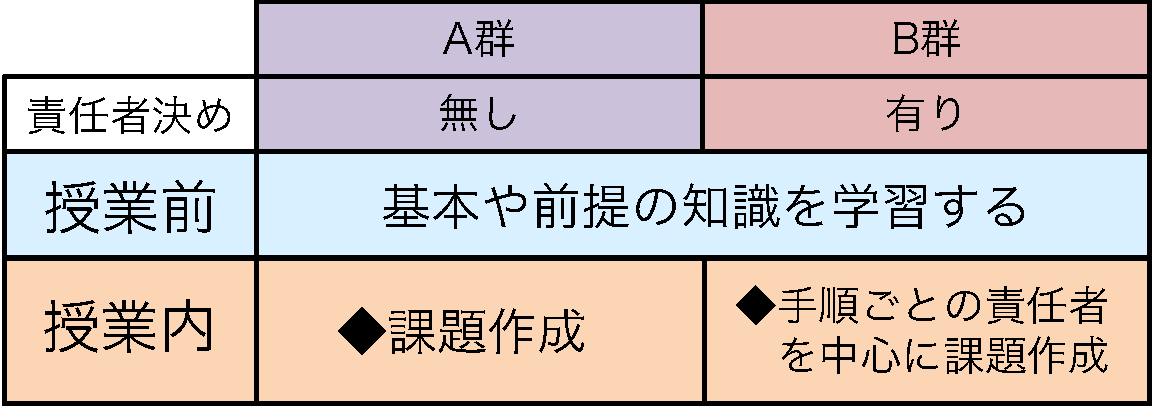
\includegraphics[clip,width=85mm,height=40mm]{nagare12.pdf}
 }
\end{center}
 \caption{責任者決め有り,無しの学習の流れ}
 \label{nagare}
\end{figure}

\newpage

\subsubsection{対象者}
本学の情報科学部情報ネットワーク学科で開講されている情報数学応用の履修者を対象にした.この内アンケートに答えたA群46名,B群52名を分析の対象にした.



\subsubsection{グループ分け方法}
グループ分け方法は両群同じ方法を取った.授業開始前に学生に,メモ用紙を取りに来てもらうタイミングと同時に番号札を配布し,その番号の1番から順に3人1グループ作成した.これに加えてB群は1番から構想,プログラミング,検証の順に責任者を決める.

\subsubsection{ハッシュ化の選択理由}
本研究では情報数学応用で行われる,ハッシュ化を対象とした.この内容を選択した理由は以下の3つである.

\begin{itemize}

 \item グループ学習として成り立つ内容
  \item 各責任者の一定作業量を確保
  \item 限られた作業時間で終わせられる内容
  
\end{itemize}




\newpage

\subsubsection{事前学習動画}
対象者に見てもらう事前学習用の動画はApple keynote作成したスライドを使用し,このスライドに「スライドショーの記録」という機能で音声を付けた動画ファイルをYouTubeで履修者のみに限定公開した.図\ref{hash-v1}や図\ref{hash-v2}のようにハッシュ関数やパスワードのハッシュ化について説明している.

\begin{figure}[h]
\begin{center}
\scalebox{1}[1.6]{
 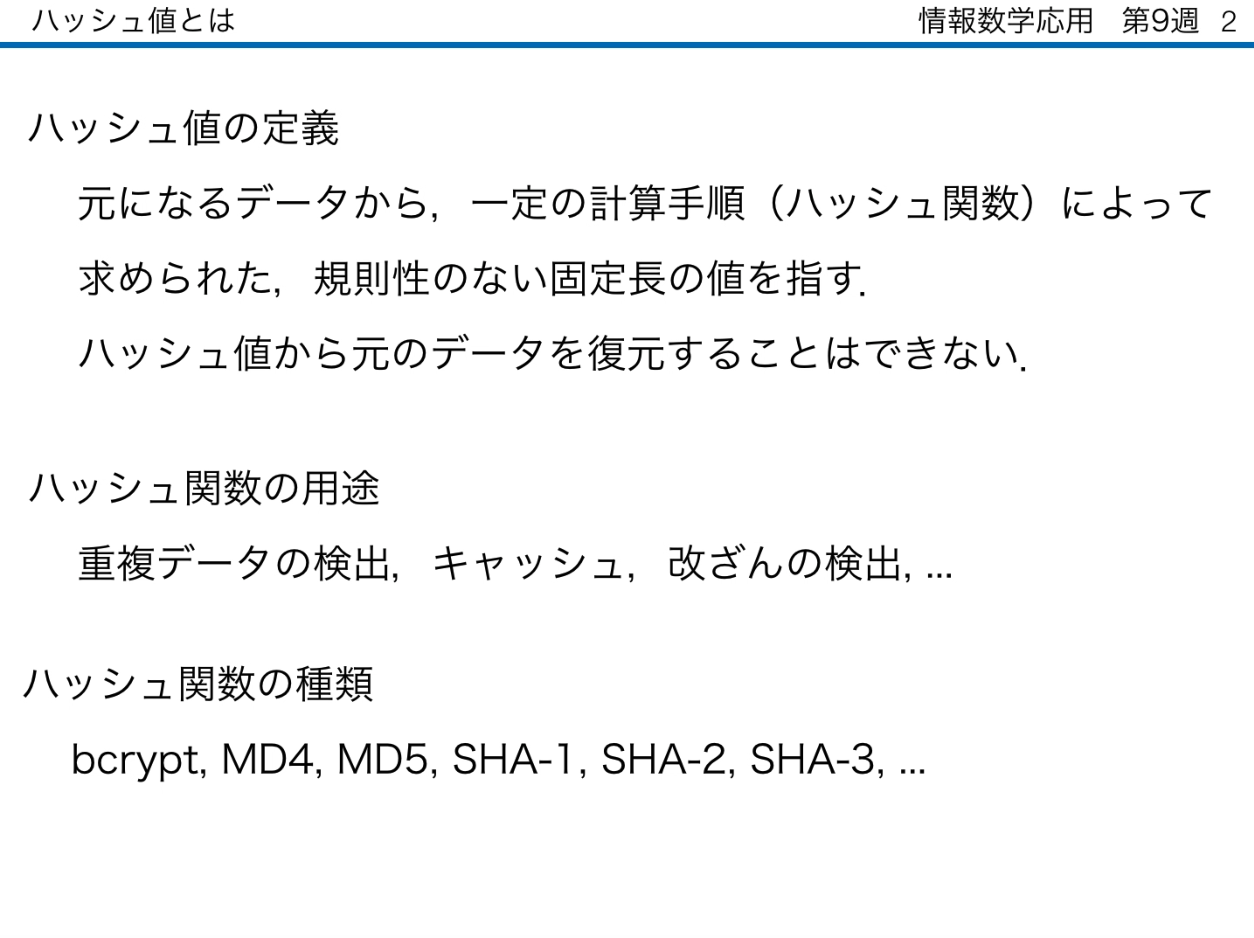
\includegraphics[clip,width=85mm,height=40mm]{hashv2.pdf}
 }
\end{center}
 \caption{事前学習動画1}
 \label{hash-v1}
\end{figure}

\begin{figure}[h]
\begin{center}
\scalebox{1}[1.6]{
 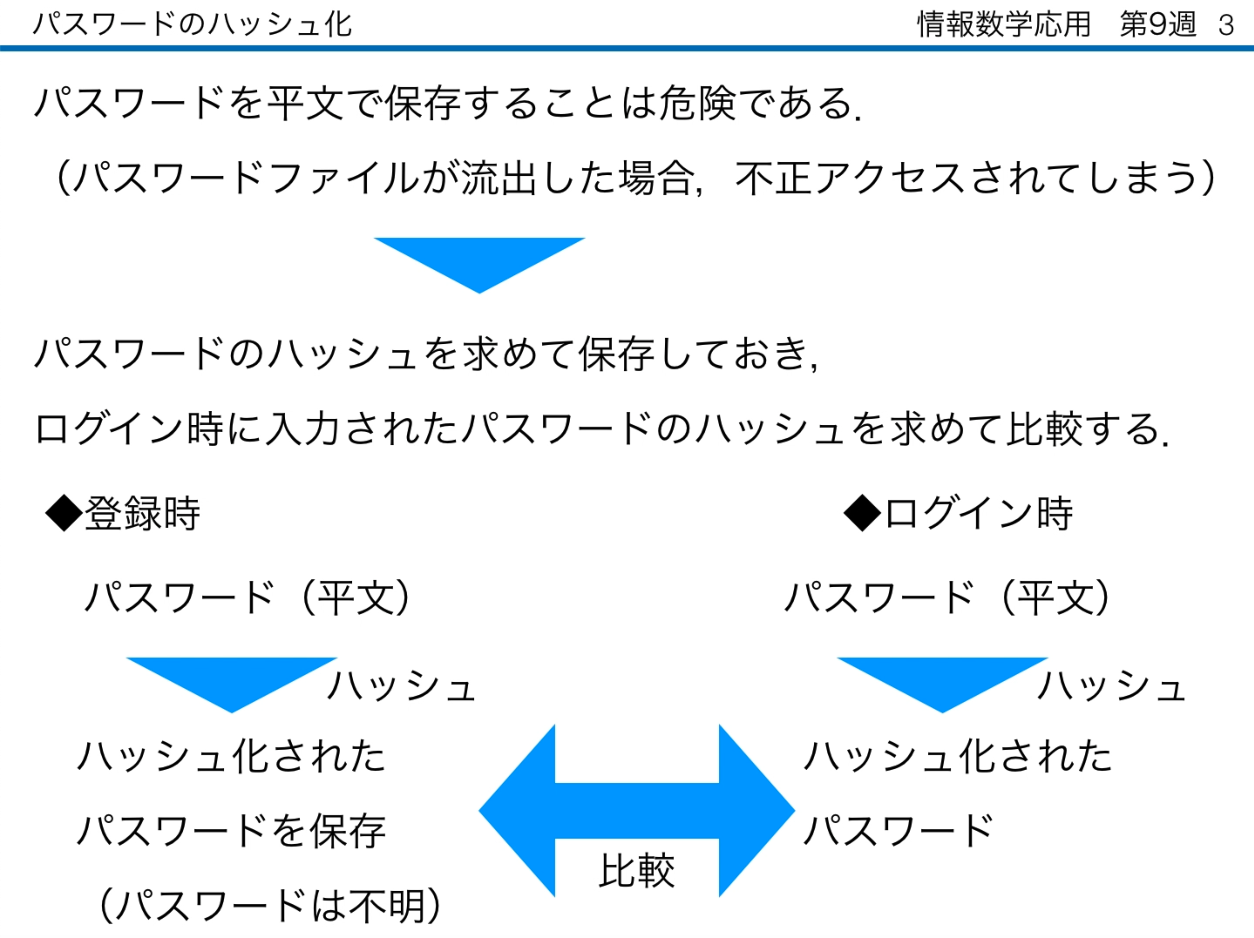
\includegraphics[clip,width=85mm,height=40mm]{hashv1.pdf}
 }
\end{center}
 \caption{事前学習動画2}
 \label{hash-v2}
\end{figure}


\newpage


\subsubsection{課題内容}
事前学習で学習した内容を定着させるため,パスワードのハッシュ化について作成課題を出した,図\ref{kadai1}は実際に出した課題である.事前学習での知識を元にグループで,擬似ログインページをプログラミングで作ってもらう.

\begin{figure}[h]
\begin{center}
\scalebox{1.5}[1.3]{
 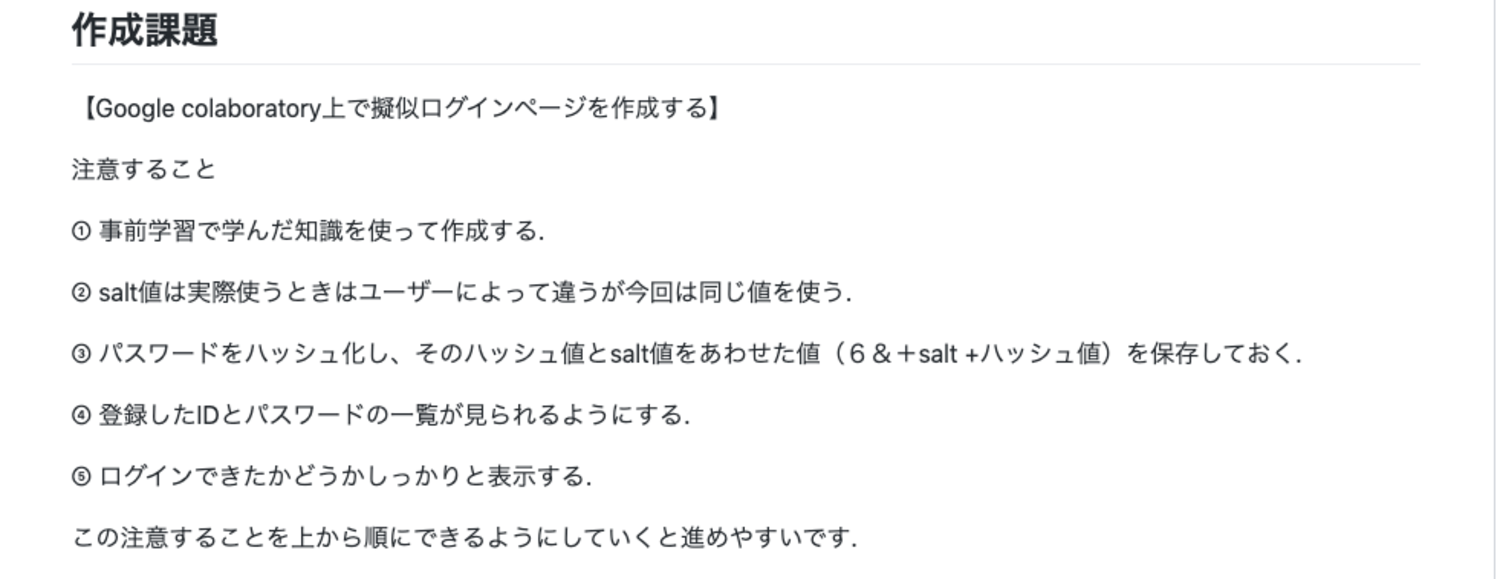
\includegraphics[clip,width=85mm,height=40mm]{kadai1.pdf}
 }
\end{center}
 \caption{作成課題(一部)}
 \label{kadai1}
\end{figure}


\subsubsection{開発環境}
開発環境は普段から利用している講義室で作業ができるようにするため,iPadでプログラミングができるGoogle Colaboratoryを選んだ.開発言語は,Google Colaboratory上で開発ができるPythonを選んだ.

\begin{description}
\item[開発端末]\mbox{}\\iPad
\item[開発環境]\mbox{}\\Google Colaboratory
\item[開発言語]\mbox{}\\Python
\end{description}

\newpage

\subsubsection{学生に教える内容}

学生に教えることと,教えないことを表\ref{osi}に示す.

学生には事前学習でハッシュ化について学んでもらう,授業内では事前学習を元に作成課題を進めてもらうので,ハッシュ化については学生に考えさせる.

Pythonで作成してもらうが事前学習ではPythonについての学習は行わない,その後の授業内での配布資料でPythonを扱う.

学生の中にはPythonに触れたことがない者もいるため,これらの資料での説明通りに進めると,課題が完成できるようになっている.

今回の反転授業で,Pyhonに関する内容を授業内で配布することにしたのは,プログラミングはこの授業で扱うハッシュ化とは違う知識だと考えたからである.

\begin{table}[htbp]
\begin{center}
\caption{学生に教える内容}
\scalebox{1.75}[1.75]{
\begin{tabular}{|c|c|c|}
\cline{1-3}
 {} & 教える&教えない \\ \cline{1-3}  
事前学習 & ハッシュ化 &Python \\ \cline{1-3}  
 授業内 & Python &ハッシュ化\\ \cline{1-3}  
\end{tabular}
}
\label{osi}
\end{center}
\end{table}

\newpage 

\subsubsection{配布資料}
グループワークをする際に学生が参考にする資料をGithub上に載せ,授業開始時に本学がで使われているmanaba上にURLを知らせる形で配布する.配布した資料の一覧を下記に示す.

\begin{description}

 \item[README.md]   \ \ \ \ \ \      グループワークの流れ
  \item[hash.ipynb]\ \ \ \ \ \ \ \ \ \ \ パスワードのハッシュ化
  \item[List.ipynb]\ \ \ \ \ \ \ \ \ \ \ \ \  辞書型
  \item[py-template.ipynb]上記以外の今回使用する知識
  
\end{description}

配布資料は全部で4つで,1つがREADME.mdでグループワークの流れやその他3つの資料のリンクが載せられている.さらに,学生の作業を進めるときにイメージがしやすいようにイメージ図\ref{kadai2}を載せて,流れの説明sita.作業する流れに加えてB群の配布資料には誰がどの作業を担当するのかが,わかりやすいようにした.

残り3つの資料は,Google Colaboratoryにテンプレートを用意して実際に動かしてPython使い方を覚えていくというものである.1つ目のhash.ipynbでハッシュ化について理解する,2つ目は辞書型と呼ばれる今回の作成に必要なものを理解してもらう,最後にPythonのifやforなどの文法の使い方を学んでもらう.

ハッシュ化を学ぶテンプレートでは,学生に事前学習動画を見た上で授業中に考える時間を与えたいので一部が空欄になっている.図\ref{kadai3}のようにパスワードのハッシュ化するときに,パスワードの平文とslatの平文を合わせたものをハッシュ化する部分を空欄とした.

これらのテンプレートを積み木のように組み合わせることで完成させることができる.



\begin{figure}[h]
\begin{center}
\scalebox{1}[1]{
 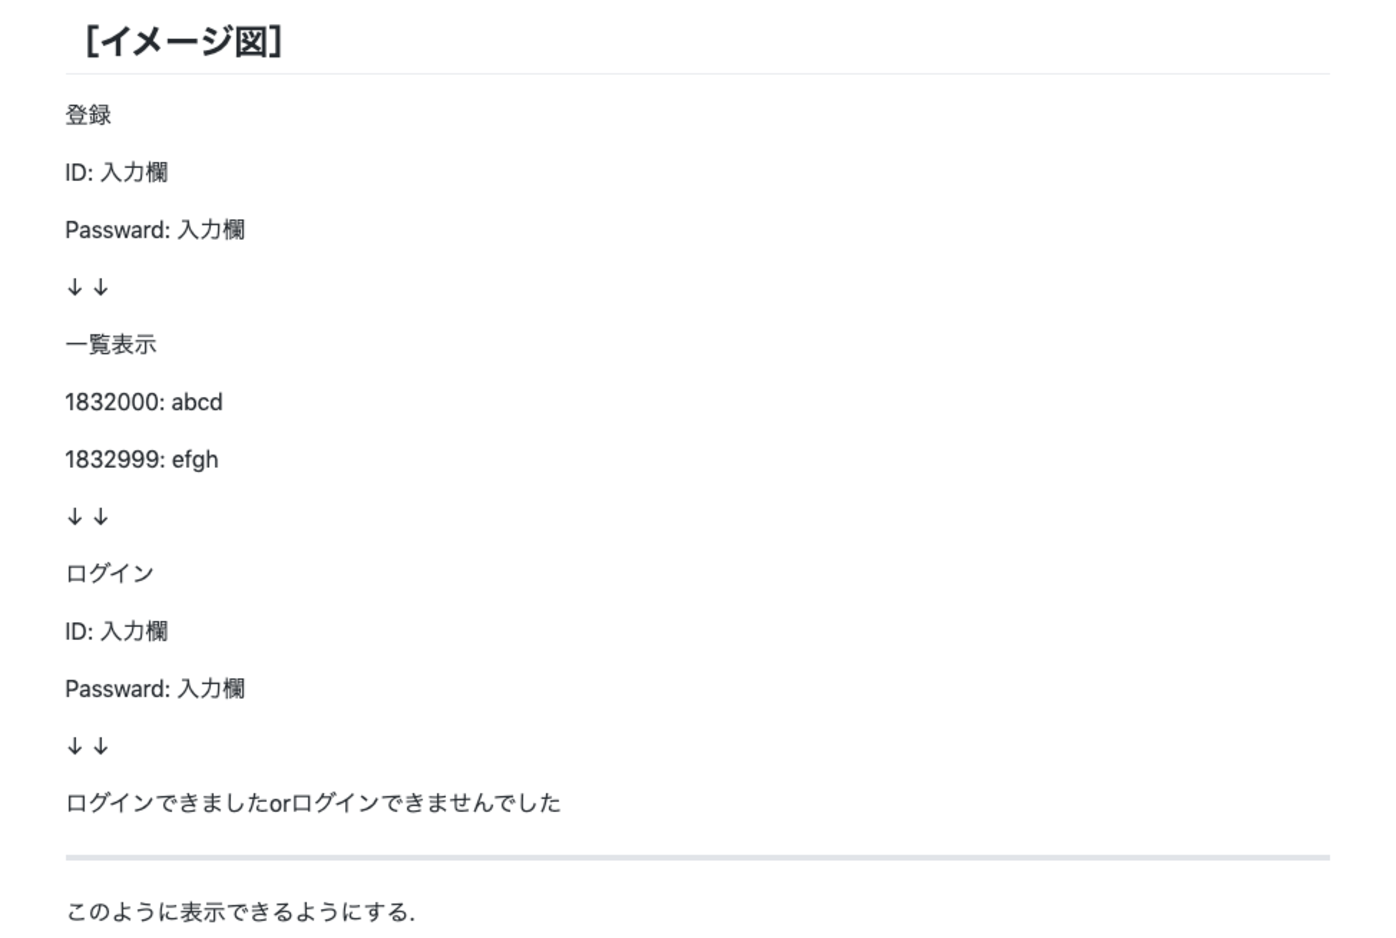
\includegraphics[clip,width=110mm]{kadai2.pdf}
 }
\end{center}
 \caption{イメージ図}
 \label{kadai2}
\end{figure}

\newpage

\begin{figure}[h]
\begin{center}
\scalebox{1}[1]{
 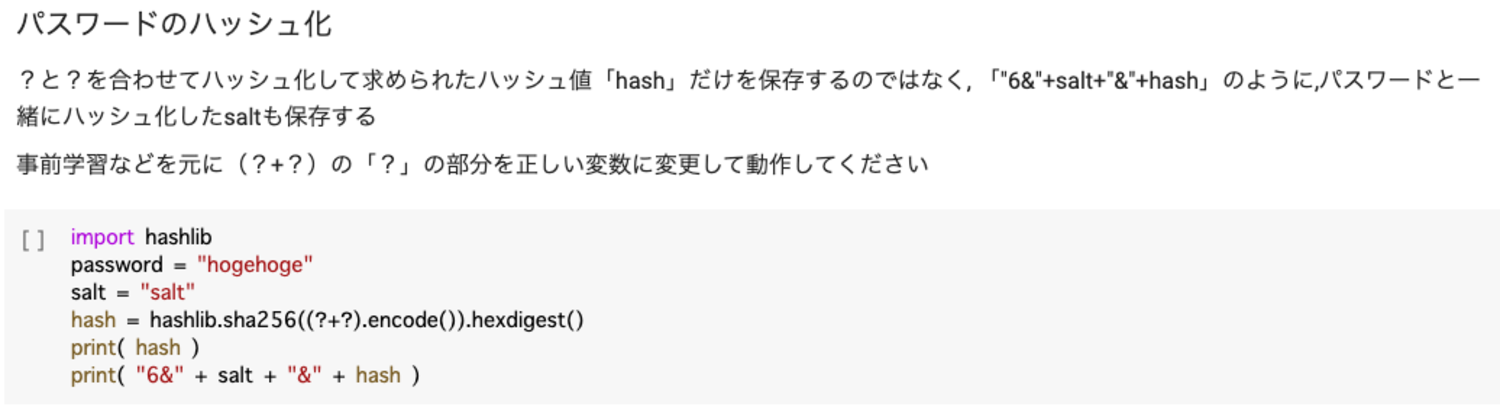
\includegraphics[clip,width=110mm]{kadai3.pdf}
 }
\end{center}
 \caption{ハッシュ化の空欄}
 \label{kadai3}
\end{figure}




\subsubsection{メモ用紙}
配布するメモ用紙(\ref{memo1})には構想,プログラミング,検証のそれぞれに自分の意見と他の人の意見を書く欄を用意した.これを使用して学生には作業を進めてもらい授業終了後に回収した.学生によっては時間内に他の人の意見を書く時間がないと考えたのでこのメモ用紙は授業自体の成績には反映させないものとした.

\begin{figure}[h]
\begin{center}
\scalebox{1}[1]{
 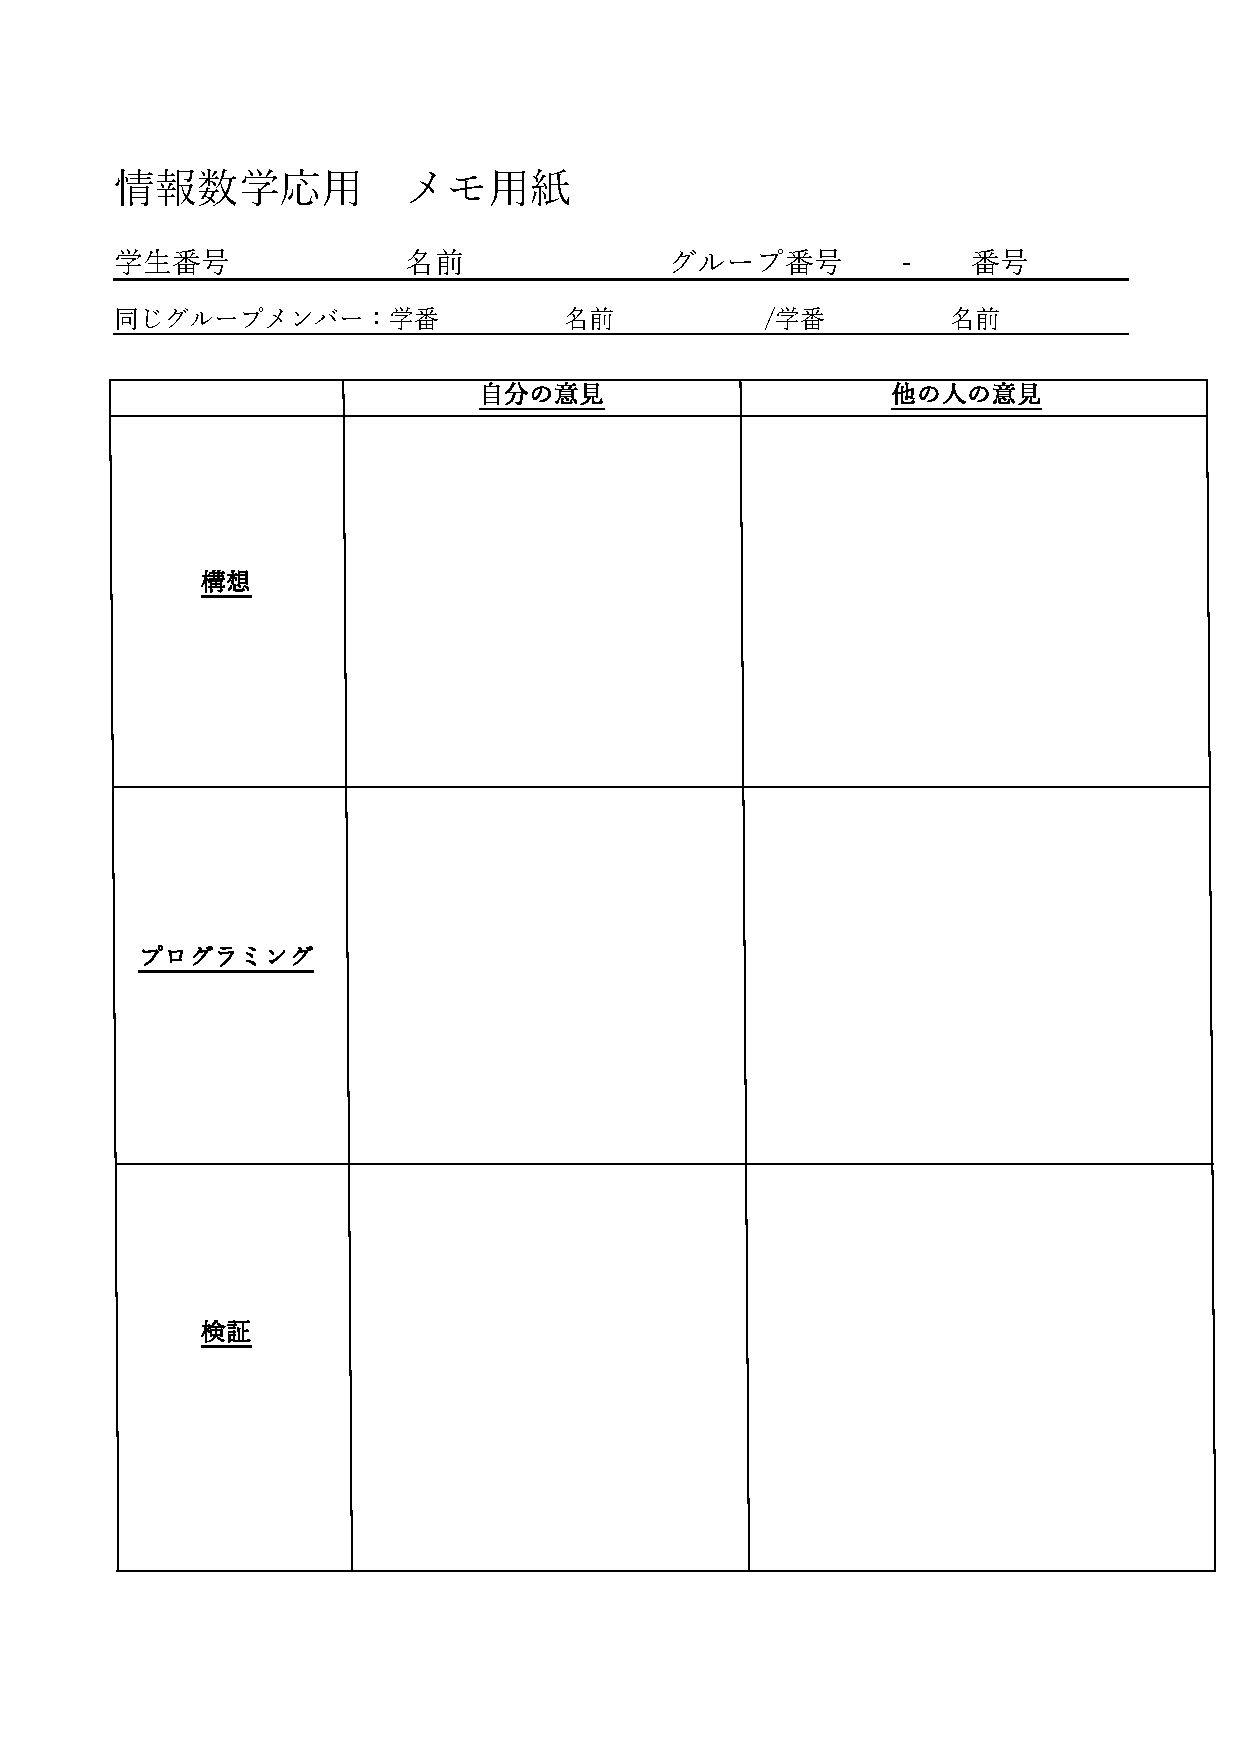
\includegraphics[clip,width=80mm]{memo1.pdf}
 }
\end{center}
 \caption{集中して事前学習に取り組めたか}
 \label{memo1}
\end{figure}
\newpage

\subsubsection{提出物}
提出物は作成したソースコードと事前学習動画などで学んだハッシュ化などについてのレポートを用意した.

\subsubsection{アンケート}
学生の主体性を調査するための項目と反転授業に関する項目を,選択式1,2問と5段階式12問,記入式2問の計16問用意し,これに加えて責任者決め有りのB群は責任者決めに関する項目を4問用意した.アンケートはGoogle Formを使って作成したものを,manabaからURLでできるようにした.

\newpage

\section{結果}
\subsection{事前学習動画に関するアンケート}
「事前学習動画を視聴したか」という質問では表\ref{anke1}のようになった.B群はA群に比べて事前学習動画をすべて視聴した学生が少ないことがわかった.


\begin{table}[htbp]
\begin{center}
\caption{事前学習動画を視聴したか(\%)}
\scalebox{1.75}[1.75]{
\begin{tabular}{|c|c|c|}
\cline{1-3}
内容 & A群 & B群  \\ \cline{1-3}  
 すべて視聴した& 78.3 & 65.4 \\ \cline{1-3}  
 ある程度視聴した& 21.7 & 32.7 \\ \cline{1-3}  
 視聴しなかった & 0 & 1.9 \\ \cline{1-3}  
\end{tabular}
}
\label{anke1}
\end{center}
\end{table}

5段階評価(1:できなかった〜5:できた)の「集中して事前学習に取り組めたか」「事前学習でメモを取れたか」「事前学習の内容を理解できたか」の3つの質問では図\ref{anke2},図\ref{anke3},図\ref{anke4}のようになった.これらの質問でもB群はA群に比べて低くなった.


\begin{figure}[h]
\begin{center}
\scalebox{1.2}[1.55]{
 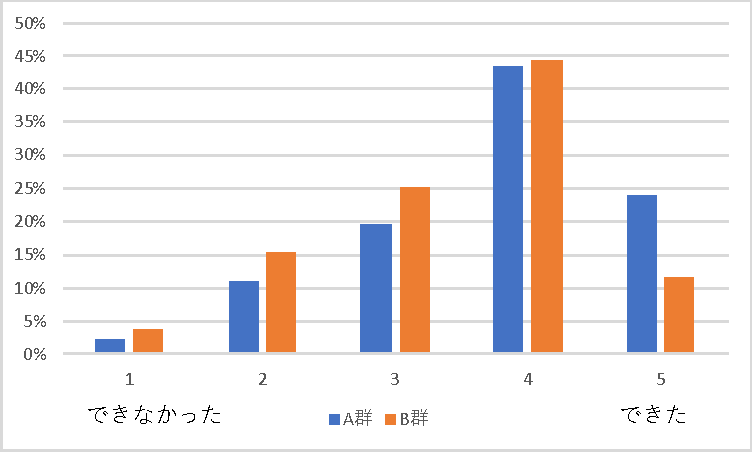
\includegraphics[clip,width=85mm,height=40mm]{anke2.pdf}
 }
\end{center}
 \caption{集中して事前学習に取り組めたか}
 \label{anke2}
\end{figure}

\newpage


\begin{figure}[h]
\begin{center}
\scalebox{1.2}[1.55]{
 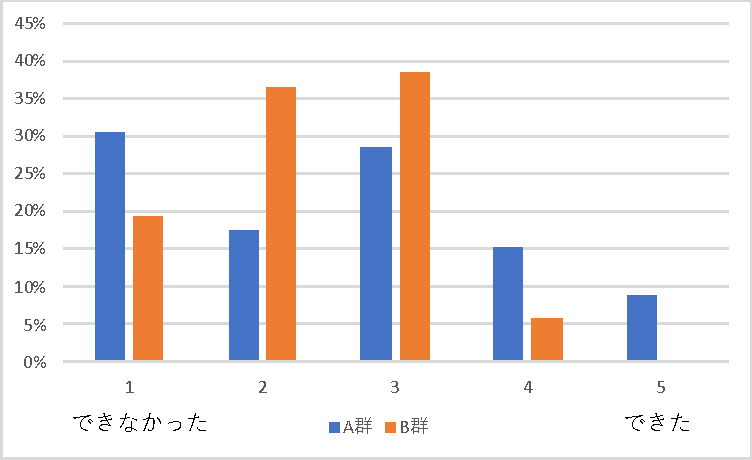
\includegraphics[clip,width=85mm,height=40mm]{anke3.pdf}
 }
\end{center}
 \caption{事前学習でメモを取れたか}
 \label{anke3}
\end{figure}


\begin{figure}[h]
\begin{center}
\scalebox{1.2}[1.55]{
 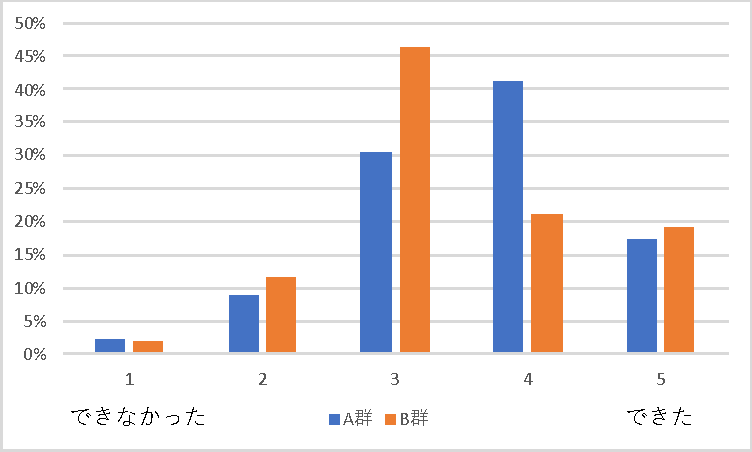
\includegraphics[clip,width=85mm,height=40mm]{anke4.pdf}
 }
\end{center}
 \caption{事前学習の内容を理解できたか}
 \label{anke4}
\end{figure}



\newpage

\subsection{課題作成に関するアンケート}
「率先して課題作成に参加できたか」という質問では図\ref{anke5}のようになった.1(できなかった)の学生は減少したが,5(できた)の学生も減少した.

\begin{figure}[h]
\begin{center}
\scalebox{1.2}[1.55]{
 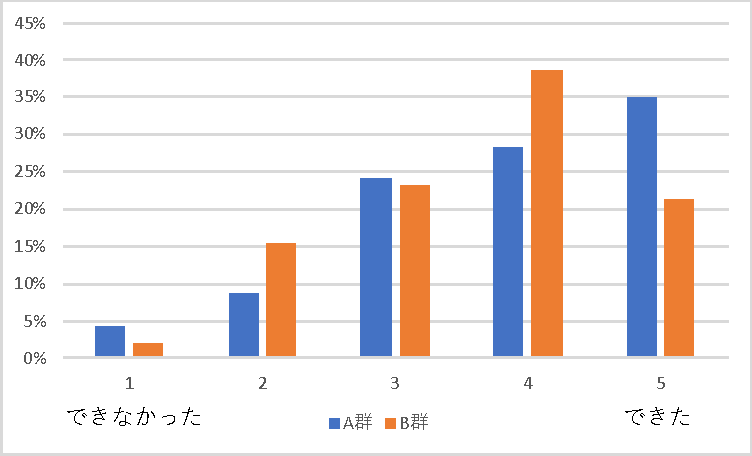
\includegraphics[clip,width=85mm,height=40mm]{anke5.pdf}
 }
\end{center}
 \caption{率先して課題作成に参加できたか}
 \label{anke5}
\end{figure}



「課題作成の中で意見を出せたか」という質問では図\ref{anke6}のようになった.5(できた)の学生が減少し,4の学生が増加した.


\begin{figure}[h]
\begin{center}
\scalebox{1.2}[1.55]{
 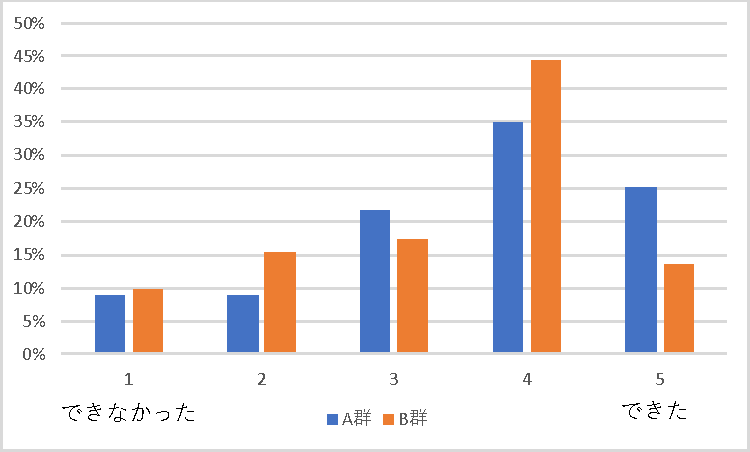
\includegraphics[clip,width=85mm,height=40mm]{anke6.pdf}
 }
\end{center}
 \caption{課題作成の中で意見を出せたか}
 \label{anke6}
\end{figure}

\newpage

「グループ全員が参加できていたか」という質問では図\ref{anke7}のようになった.1(できなかった)の学生は減少したが,5(できた)の学生も減少した.


\begin{figure}[h]
\begin{center}
\scalebox{1.2}[1.55]{
 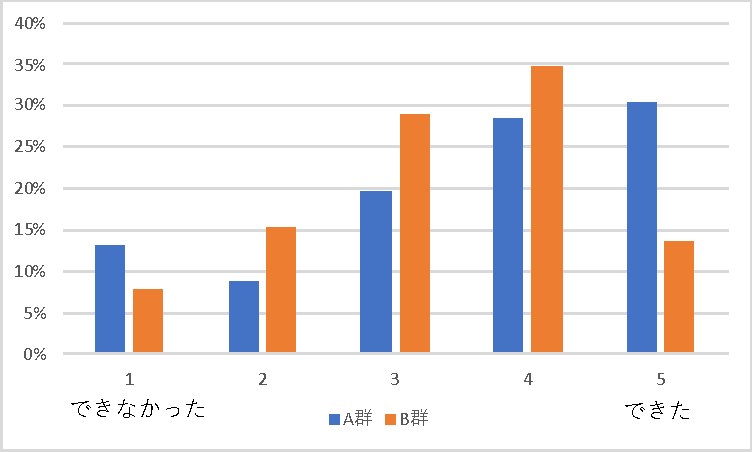
\includegraphics[clip,width=85mm,height=40mm]{anke7.pdf}
 }
\end{center}
 \caption{グループ全員が参加できていたか}
 \label{anke7}
\end{figure}



「主体的に取り組むことができたか」という質問では図\ref{anke8}のようになった.1(できなかった)の学生は減少したが,5(できた)の学生も減少した.だが,4と5を合計した数値がA群よりもB群のほうがわずかに増加した.

\begin{figure}[h]
\begin{center}
\scalebox{1.2}[1.55]{
 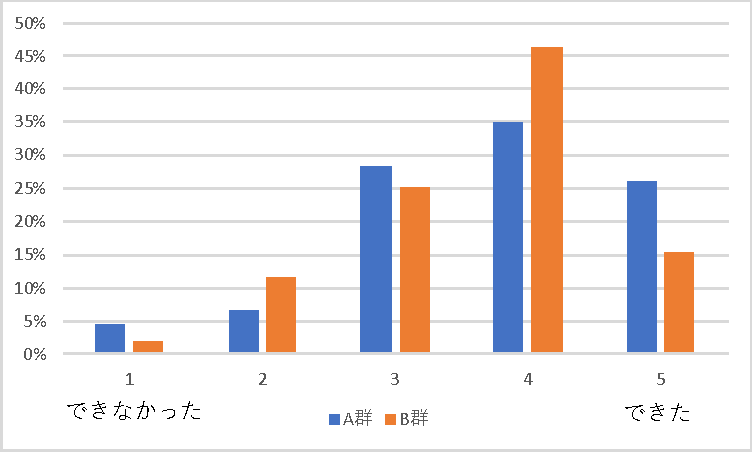
\includegraphics[clip,width=85mm,height=40mm]{anke8.pdf}
 }
\end{center}
 \caption{主体的に取り組むことができたか}
 \label{anke8}
\end{figure}



\newpage
\subsection{反転授業に関するアンケート}

「普段の講義に比べて主体的に取り組めたか」という質問では図\ref{anke9}のようになった.1(できなかった)と5(できた)が減少した.

\begin{figure}[h]
\begin{center}
\scalebox{1.2}[1.55]{
 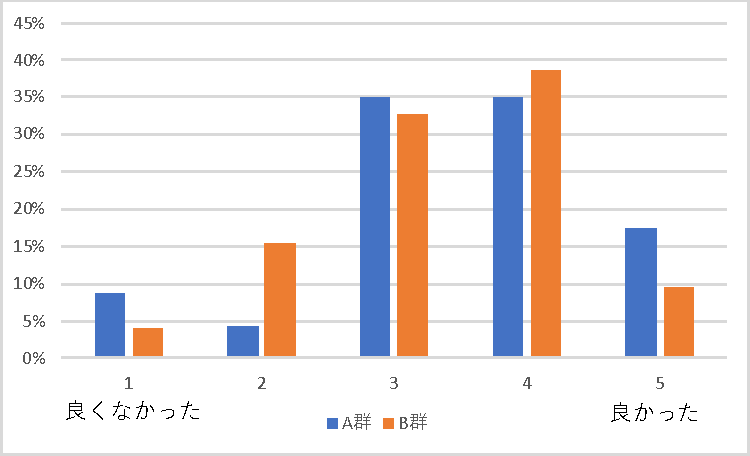
\includegraphics[clip,width=85mm,height=40mm]{anke9.pdf}
 }
\end{center}
 \caption{普段の講義に比べて主体的に取り組めたか}
 \label{anke9}
\end{figure}

「反転授業をやってみてよかったか」という質問では図\ref{anke10}のようになった.この質問では2と3が増加した.

\begin{figure}[h]
\begin{center}
\scalebox{1.2}[1.55]{
 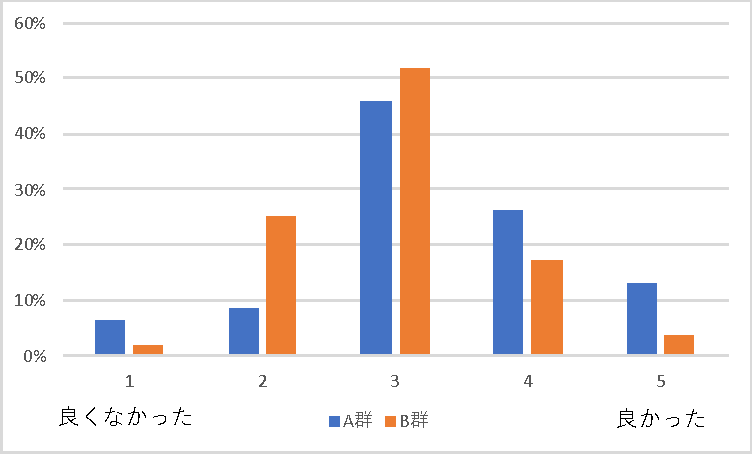
\includegraphics[clip,width=85mm,height=40mm]{anke10.pdf}
 }
\end{center}
 \caption{反転授業をやってみてよかったか}
 \label{anke10}
\end{figure}

\newpage
「今後も反転授業をやってみたいか」という質問では図\ref{anke11}のようになった.今後もやってみたいと考える学生は少なかった.

\begin{figure}[h]
\begin{center}
\scalebox{1.2}[1.55]{
 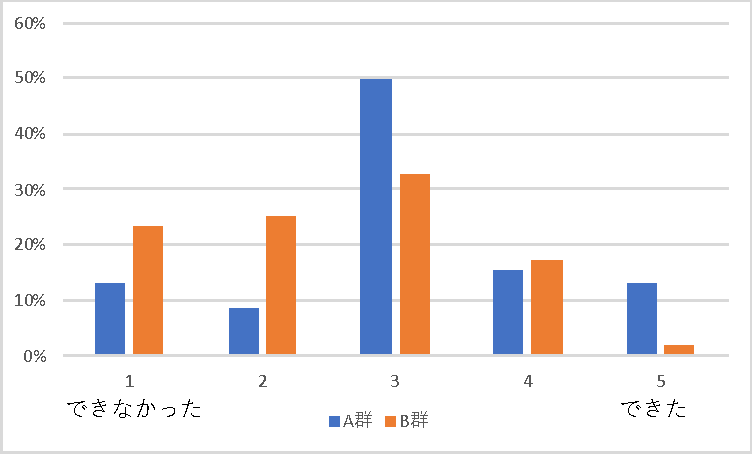
\includegraphics[clip,width=85mm,height=40mm]{anke11.pdf}
 }
\end{center}
 \caption{今後も反転授業をやってみたいか}
 \label{anke11}
\end{figure}

「他の授業でも反転授業をやってみたいか」という質問では図\ref{anke12}のようになった.他の授業でもやってみたいと考える学生は少なかった.

\begin{figure}[h]
\begin{center}
\scalebox{1.2}[1.55]{
 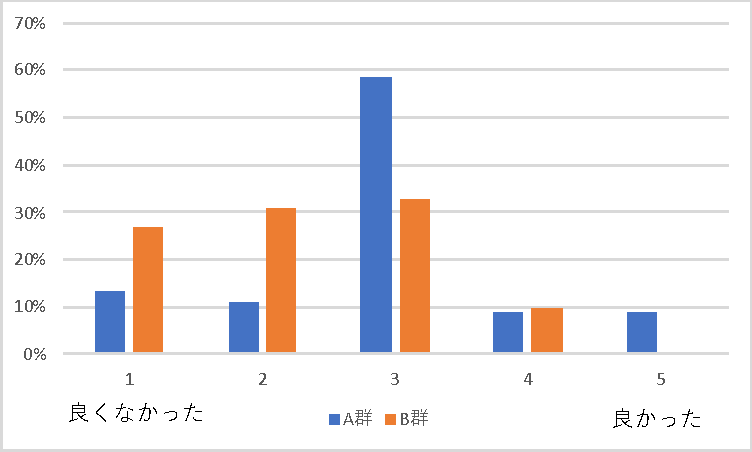
\includegraphics[clip,width=85mm,height=40mm]{anke12.pdf}
 }
\end{center}
 \caption{他の授業でも反転授業をやってみたいか}
 \label{anke12}
\end{figure}

\newpage
「通常の授業に比べて理解度は上がったか」という質問では図\ref{anke13}のようになった.1(できなかった)の学生は減少したが,5(できた)の学生も減少した.

\begin{figure}[h]
\begin{center}
\scalebox{1.2}[1.55]{
 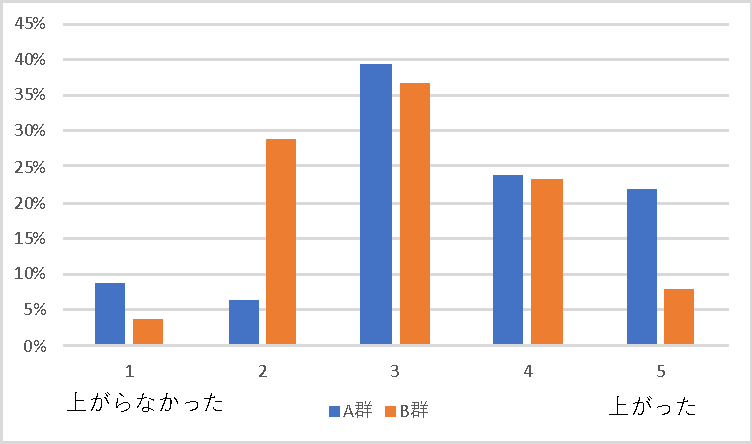
\includegraphics[clip,width=85mm,height=40mm]{anke13.pdf}
 }
\end{center}
 \caption{通常の授業に比べて理解度は上がったか}
 \label{anke13}
\end{figure}


\newpage
\subsection{責任者を決めたクラス(B群)のみにしたアンケート}

「あなたが責任者のときに主体的に課題に取り組めたか」という質問では図\ref{anke14}のようになった.できなかった学生よりはできた学生の方が多かった

\begin{figure}[h]
\begin{center}
\scalebox{1.2}[1.55]{
 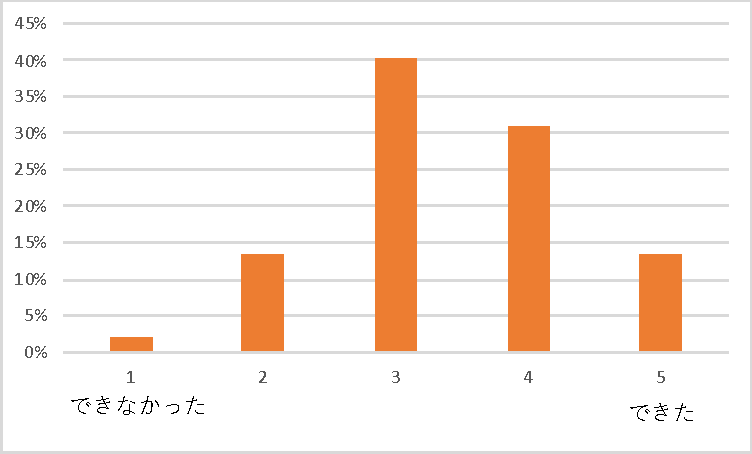
\includegraphics[clip,width=85mm,height=40mm]{anke14.pdf}
 }
\end{center}
 \caption{あなたが責任者のときに主体的に課題に取り組めたか}
 \label{anke14}
\end{figure}

「責任者の指示に従い取り組めたか」という質問では図\ref{anke15}のようになった.4に票が集中した.

\begin{figure}[h]
\begin{center}
\scalebox{1.2}[1.55]{
 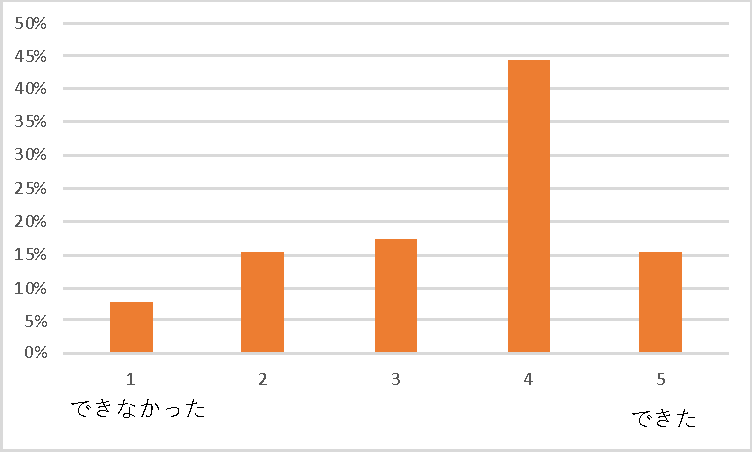
\includegraphics[clip,width=85mm,height=40mm]{anke15.pdf}
 }
\end{center}
 \caption{責任者の指示に従い取り組めたか}
 \label{anke15}
\end{figure}


\newpage

「あなた以外が責任者だったときその人は責任者として取り組めていたか」という質問では図\ref{anke16}のようになった.1を選んだ学生が少なかった.

\begin{figure}[h]
\begin{center}
\scalebox{1.2}[1.55]{
 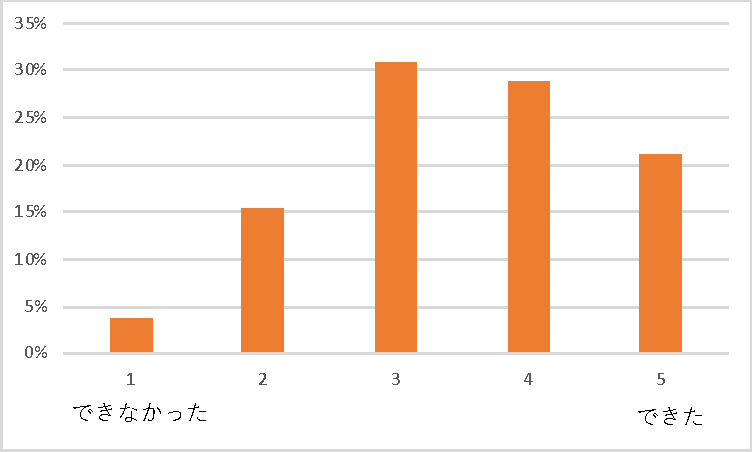
\includegraphics[clip,width=85mm,height=40mm]{anke16.pdf}
 }
\end{center}
 \caption{あなた以外が責任者だったときその人は責任者として取り組めていたか}
 \label{anke16}
\end{figure}

「責任者ではないときも意見を出すことができたか」という質問では図\ref{anke17}のようになった.1.2を選ぶ学生は少なかった.

\begin{figure}[h]
\begin{center}
\scalebox{1.2}[1.55]{
 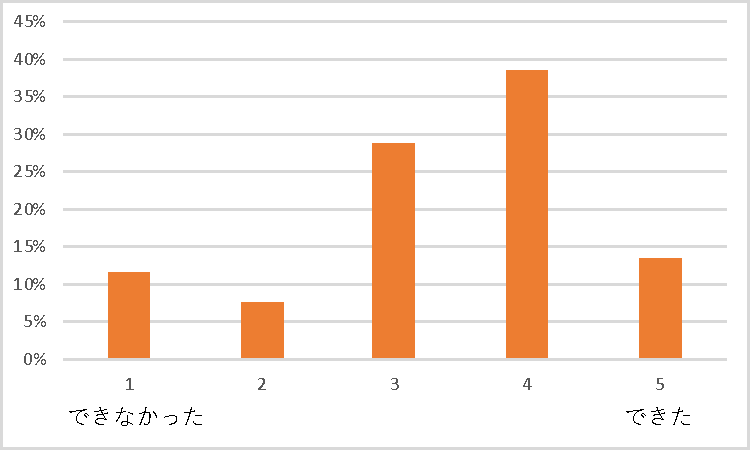
\includegraphics[clip,width=85mm,height=40mm]{anke17.pdf}
 }
\end{center}
 \caption{責任者ではないときも意見を出すことができたか}
 \label{anke17}
\end{figure}


\newpage
\subsection{記述欄}
2つ記述欄を用意したところ以下のような回答が書かれた.

課題作成の中で「どのようにしたらもっと良いものができたか」という質問内容では表\ref{anke18}のような回答が出た.

\begin{table}[htbp]
\begin{center}
\caption{どのようにしたらもっと良いものができたか}
\scalebox{1}[1]{
\begin{tabular}{|c|c|c|}
\cline{1-2}
\multicolumn{1}{|c|}{\multirow{2}{*}{A群}} & 意見交換を率先して行う   \\ \cline{2-2}  
\multicolumn{1}{|c|}{} &  既知の言語でやれば早く多く意見交換も進んだ \\ \cline{2-2}  
\multicolumn{1}{|c|}{} &  構想したものをいろいろと試してみればよかった \\ \cline{2-2}  
\multicolumn{1}{|c|}{} &  事前の課題説明 \\ \cline{2-2} 
\multicolumn{1}{|c|}{} &  技術的な改善点(プログラミング) \\ \cline{1-2} 
 \multicolumn{1}{|c|}{\multirow{2}{*}{B群}} & 事前学習をもっとしっかりやっておけばよかった  \\ \cline{2-2}  
\multicolumn{1}{|c|}{} & 時間が足りなかった  \\ \cline{2-2}  
\multicolumn{1}{|c|}{} & もっと意見交換のやりやすい場所,グループ形態 \\ \cline{2-2}  
\multicolumn{1}{|c|}{} & もっと意見交換をすればよかった  \\ \cline{2-2}  
\multicolumn{1}{|c|}{} & 既知の言語での開発  \\ \cline{2-2}  
\multicolumn{1}{|c|}{} & Pythonの知識をもっとつけておけばよかった  \\ \cline{1-2}  
\end{tabular}
}
\label{anke18}
\end{center}
\end{table}

反転授業をやってみた感想を尋ねたところ,表\ref{anke18}のような回答が出た.


\begin{table}[htbp]
\begin{center}
\caption{感想}
\scalebox{1}[1]{
\begin{tabular}{|c|c|c|}
\cline{1-2}
\multicolumn{1}{|c|}{\multirow{2}{*}{A群}} &  事前に映像で学習できたのがよかった  \\ \cline{2-2}  
\multicolumn{1}{|c|}{} & 座学での講義よりも集中して取り組むことができた  \\ \cline{2-2}  
\multicolumn{1}{|c|}{} & 時間が足りなかった  \\ \cline{2-2}  
\multicolumn{1}{|c|}{} & 演習室でやりたかった  \\ \cline{2-2}  
\multicolumn{1}{|c|}{} & 登録やログインなどの身近なプログラムに触れることができて楽しかった \\ \cline{2-2} 
\multicolumn{1}{|c|}{} &  ほかの人の意見も参考にすることができ、いい勉強になった \\ \cline{2-2} 
\multicolumn{1}{|c|}{} &  反転授業とは? \\ \cline{1-2} 
 \multicolumn{1}{|c|}{\multirow{2}{*}{B群}} & 時間が足りなかった  \\ \cline{2-2}  
\multicolumn{1}{|c|}{} & 反転授業とは?  \\ \cline{2-2}  
\multicolumn{1}{|c|}{} & 他人を絡めることで責任感が出るのでよかった \\ \cline{2-2}  
\multicolumn{1}{|c|}{} &  iPadでプログラミングをするのはとても大変で作業が進みずらかった \\ \cline{2-2}  
\multicolumn{1}{|c|}{} &  普段の授業よりも考える時間が多かったので良かった \\ \cline{2-2}  
\multicolumn{1}{|c|}{} &  誰かと共有することで深く考えることができた気がした \\ \cline{2-2}  
\multicolumn{1}{|c|}{} & もう少し人数を増やして欲しかった  \\ \cline{2-2}  
\multicolumn{1}{|c|}{} & 動画を観ていない人が多く居て、円滑な進行ができなかった  \\ \cline{1-2}  
\end{tabular}
}
\label{anke18}
\end{center}
\end{table}



\newpage
\section{考察と今後の課題}
\subsection{反転授業への慣れ}
今回実験を行った本学の学生は,反転授業をやったことがなかった.そのため,事前学習動画を見てくるという流れができなかった学生がいた可能性がある.

反転授業という今までやってきた学習とは,逆のことをするという学習方法が,すぐには受け入れられなかったと考えられる.よって,事前学習動画の視聴率を上げるために,対象者に対して反転授業を数回繰り返す必要があると考えた.
\subsection{作業時間}
学生からの記述回答で「時間が足りなかった」という回答が多く出た.B群は特にそれぞれの役割を中心に考える時間を要するため,グループで作業を進める時間が足りなくなってしまったと考えられる.これを改善するために講義2回分にして行うか,課題内容を調整し時間内に終わらせられるようにする必要がある.

例えば,本研究では積み木のように,複数のテンプレートを組み合わせることで完成することができたが,そうではなく,ハッシュ化していない疑似ログインページのソースコードを配布し,これを学生の手でハッシュ化したパスワードを保存するログインページに,改良するという方法も考える.

\subsection{場所}
今回の授業では普段から利用している生徒が横並びになる講義室で行った.しかし,意見交換する際に隣の人以外と会話をしにくい環境であった.グループワークがもっとやりやすくなるように学生が向かい合わせになるような場所を選ぶべきであった.

\subsection{開発環境}
学生から「既知の言語での開発がしたかった」という意見が出たが,今回は,他の授業で演習室が使えないという状況で,行わないといけなかったためiPadでの開発になり,iPadで開発言語で行う必要があった.また,現在iPadで開発できる言語は数多くあるが,学生の導入の私易さ,提出方法などを加味した結果,Google ColaboratoryでPythonを選択した.
そのため,学生の導入の私易さや提出方法などを考慮した,開発ツールが生み出されることでc言語やJavaの様な言語の開発が行えるようになる.



\newpage
\section{結言}
近年では,時代の変化がとても早い中で主体性を持ち自ら学び,考え,行動できる人材が必要とされている.しかし,教育の場では受動的な学習が行われている.その原因の1つとして学生の主体性が低いことが挙げられる.そこで,主体性を持って学習が行えるようになる方法の1つとして反転授業が注目されている.予習動画すべて見る学生が少ないなど,グループ学習を取り入れた反転授業では元から主体性が持つ学生だけで進めてしまう.これらのように,学習者の主体性の違いが問題とされている.

そこで本研究では反転授業のグループ学習において,一人一人の学生に責任ある立場に付かせてグループワークを行ってもらい,主体性に変化があったかを分析することを目的とした.しかし,本研究で行った実験だけでは学生の主体性に違いは見られなかった.だが,改善点が見つかったため,本研究での方法が間違っているとは断定できないという結果となった.


\newpage
\section*{謝辞}
\addcontentsline{toc}{section}{謝辞}
本研究の進行および本論文の作成にあたり,多くの御助言と御指導いただきました須田宇宙准教授に深く感謝の意を表します.また実験に協力して頂いた情報数学応用の受講者に深く感謝の意を表します.
\newpage

\bibliographystyle{jplain}
\addcontentsline{toc}{section}{参考文献}
\begin{thebibliography}{3}
\bibitem{1}三田満男「反転授業の実践とその課題」日本医療科学大学,日本科学教育研究会研究報告,Vol.31,No.5,(2017),2019/8/25参照
\bibitem{2}大谷千恵,田村恵理子,河野功幸,根津幸徳,池田敦 「文系授業における反転授業の事例研究」玉川大学教育学部紀要 第17号 2017, pp117~142,2019/10/25参照
\bibitem{3}見坊豪紀,金田一春彦,柴田武,山田忠雄,金田一京助「新明解国語辞典 第三版」株式会社三省堂,1989年,pp531,2019/11/21参照
\bibitem{4}経済産業省「社会人基礎力」https://www.meti.go.jp/policy/kisoryoku/,2020/1/9参照
\bibitem{5}一般社団法人 日本経済団体連合会「高等教育に関するアンケート調査結果」http://www.keidanren.or.jp/policy/2018/029.html,2020/1/9参照
\bibitem{6}ベネッセ教育総合研究所「第3回 大学生の学習・生活実態調査報告書」https://berd.benesse.jp/koutou/research/detail1.php?id=5169
\end{thebibliography}

\newpage
\section*{付録}
\addcontentsline{toc}{section}{付録}


\end{document}